\cmfnewsection{Exportando Dados}{./logos/fundo_tese}{0.15}






%%%%%%%%%%%%%%%%%%%%%%%%%%%%%%%%%%%%%%%%%%%%%%%%
%%%%%%%%%%%%%%%%%%%%%%%%%%%%%%%%%%%%%%%%%%%%%%%%
%%%%%%%%%%%%%%%%%%%%%%%%%%%%%%%%%%%%%%%%%%%%%%%%
%%%%%%%%%%%%%%%%%%%%%%%%%%%%%%%%%%%%%%%%%%%%%%%%
\begin{frame}{Porque Exportar Dados?}
\centering


\textbf{Motivo 1:} Para produzir gráficos com melhor qualidade 
\vspace*{1cm}

\begin{columns}

\column{0.5\linewidth}
\centering
\textbf{PSCAD}
\vspace*{0.5cm}

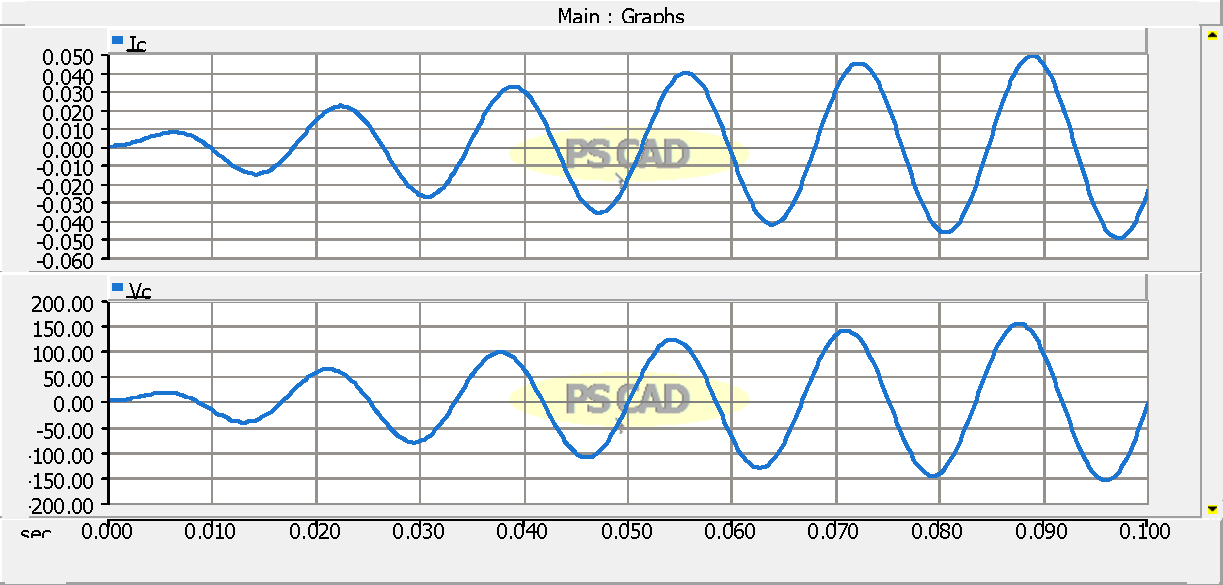
\includegraphics[width=0.90\linewidth]{./figuras/Exportacao/ex_pscadfig}
\column{0.5\linewidth}
\centering
\textbf{MATLAB/OCTAVE/matplotlib/etc}
\vspace*{0.5cm}

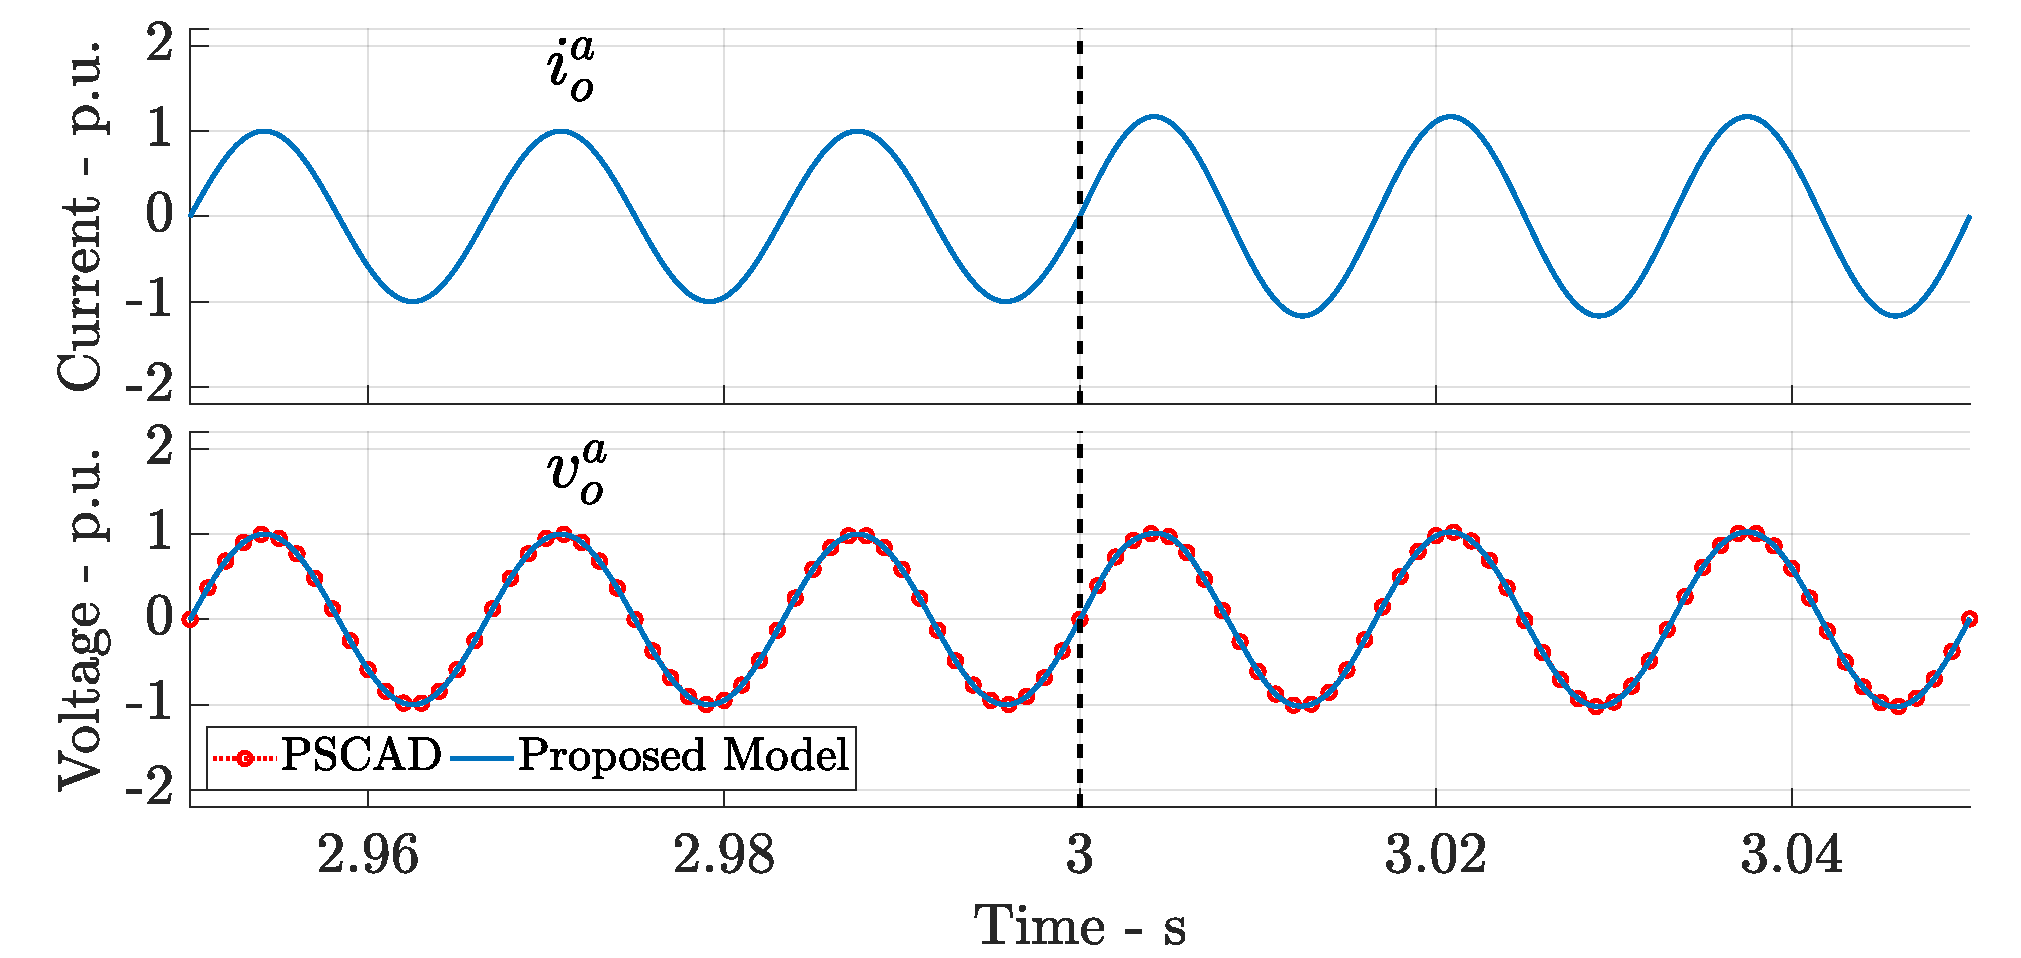
\includegraphics[width=0.90\linewidth]{./figuras/Exportacao/ex_matlab}

\end{columns}

\end{frame}





%%%%%%%%%%%%%%%%%%%%%%%%%%%%%%%%%%%%%%%%%%%%%%%%
%%%%%%%%%%%%%%%%%%%%%%%%%%%%%%%%%%%%%%%%%%%%%%%%
%%%%%%%%%%%%%%%%%%%%%%%%%%%%%%%%%%%%%%%%%%%%%%%%
%%%%%%%%%%%%%%%%%%%%%%%%%%%%%%%%%%%%%%%%%%%%%%%%
\begin{frame}{Porque Exportar Dados?}
\centering


\textbf{Motivo 2:} Para produzir gráficos de variáveis/funções indiretamente obtidas
\vspace*{1cm}

\textbf{Diagrama de bode}
\vspace*{0.5cm}

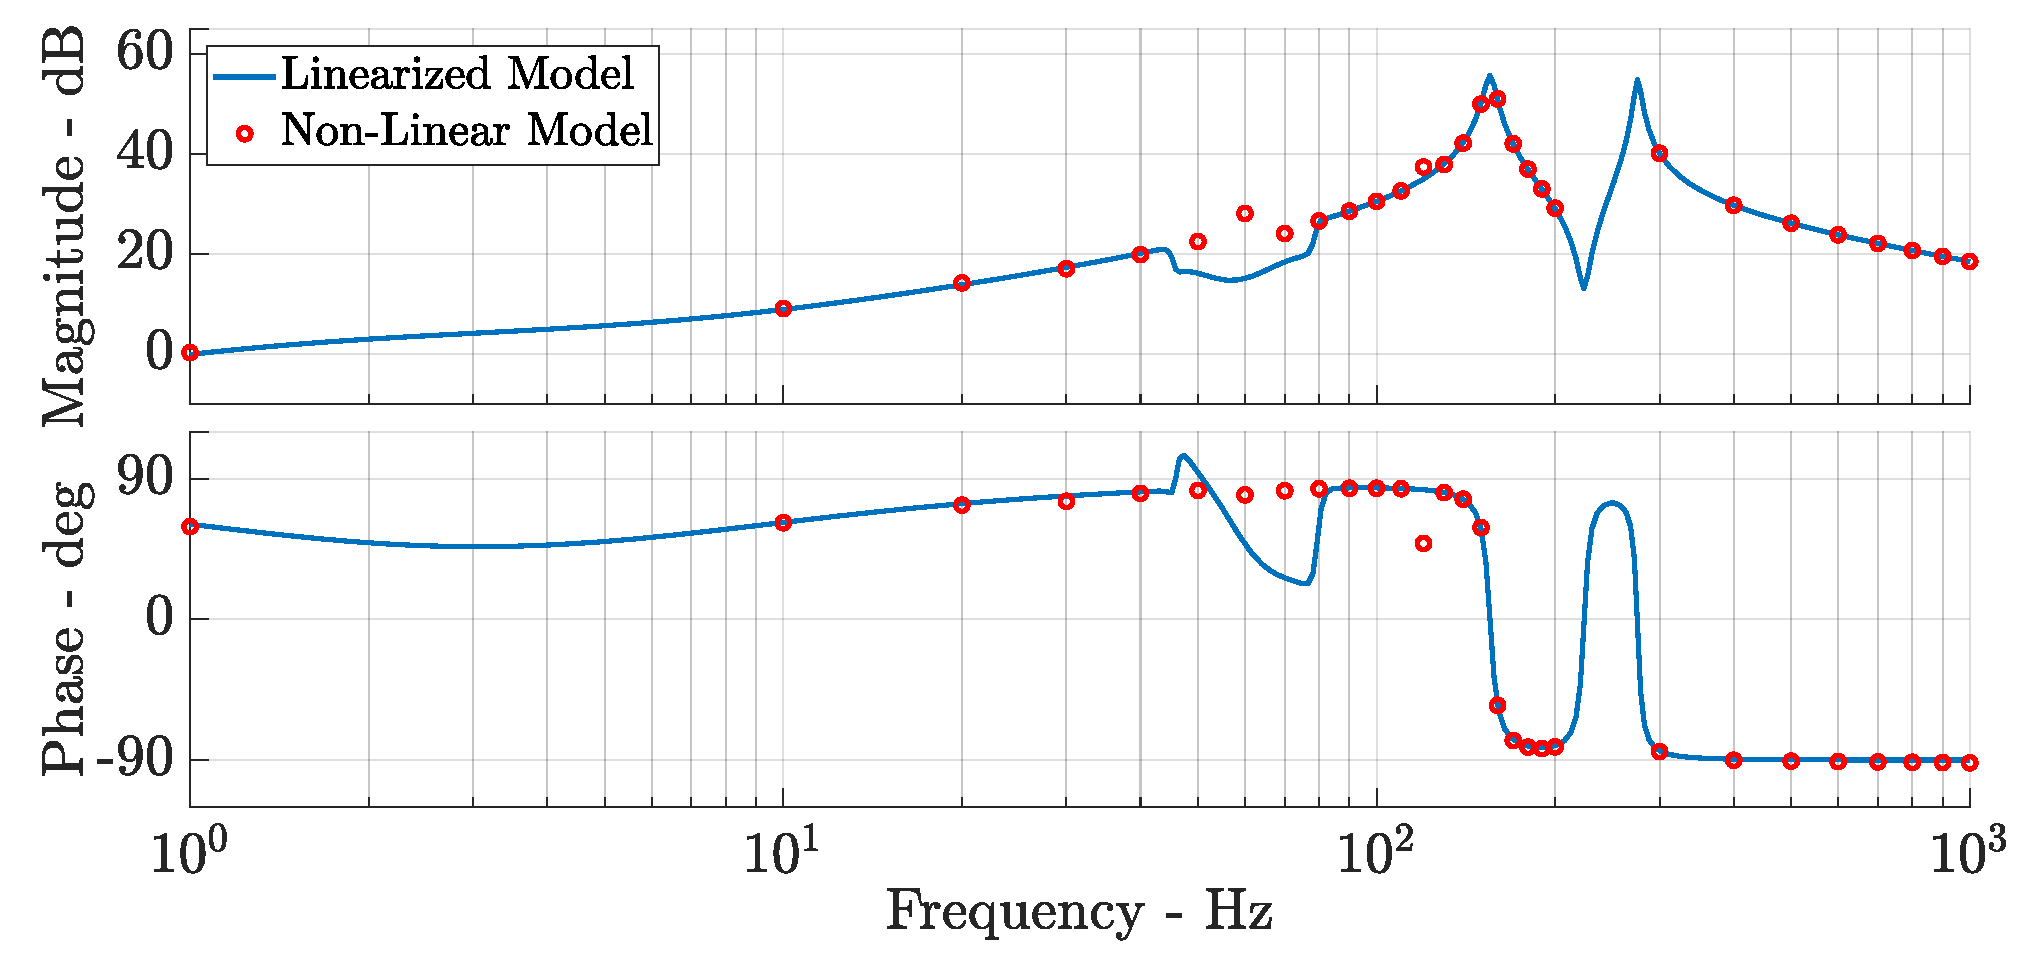
\includegraphics[width=0.60\linewidth]{./figuras/Exportacao/ex_indireto}

\end{frame}






%%%%%%%%%%%%%%%%%%%%%%%%%%%%%%%%%%%%%%%%%%%%%%%%
%%%%%%%%%%%%%%%%%%%%%%%%%%%%%%%%%%%%%%%%%%%%%%%%
%%%%%%%%%%%%%%%%%%%%%%%%%%%%%%%%%%%%%%%%%%%%%%%%
%%%%%%%%%%%%%%%%%%%%%%%%%%%%%%%%%%%%%%%%%%%%%%%%
\begin{frame}{Porque Exportar Dados?}
\centering


\textbf{Motivo 3:} Para Processar Dados
\vspace*{0.5cm}

\textbf{Ex:} Extração de componentes simétricas no domínio do tempo\footnote[frame]{\tiny Verônica Rodrigues Feijão, \href{https://drive.google.com/file/d/1xZGZLela_iNW0KIjTQ59YyCL1-sb16IO/view}{Estudo de Localização de Faltas de Curta Duração para uma Rede de 14 Barras}. Projeto de Graduação -  UERJ, 2019.}
\vspace*{0.5cm}

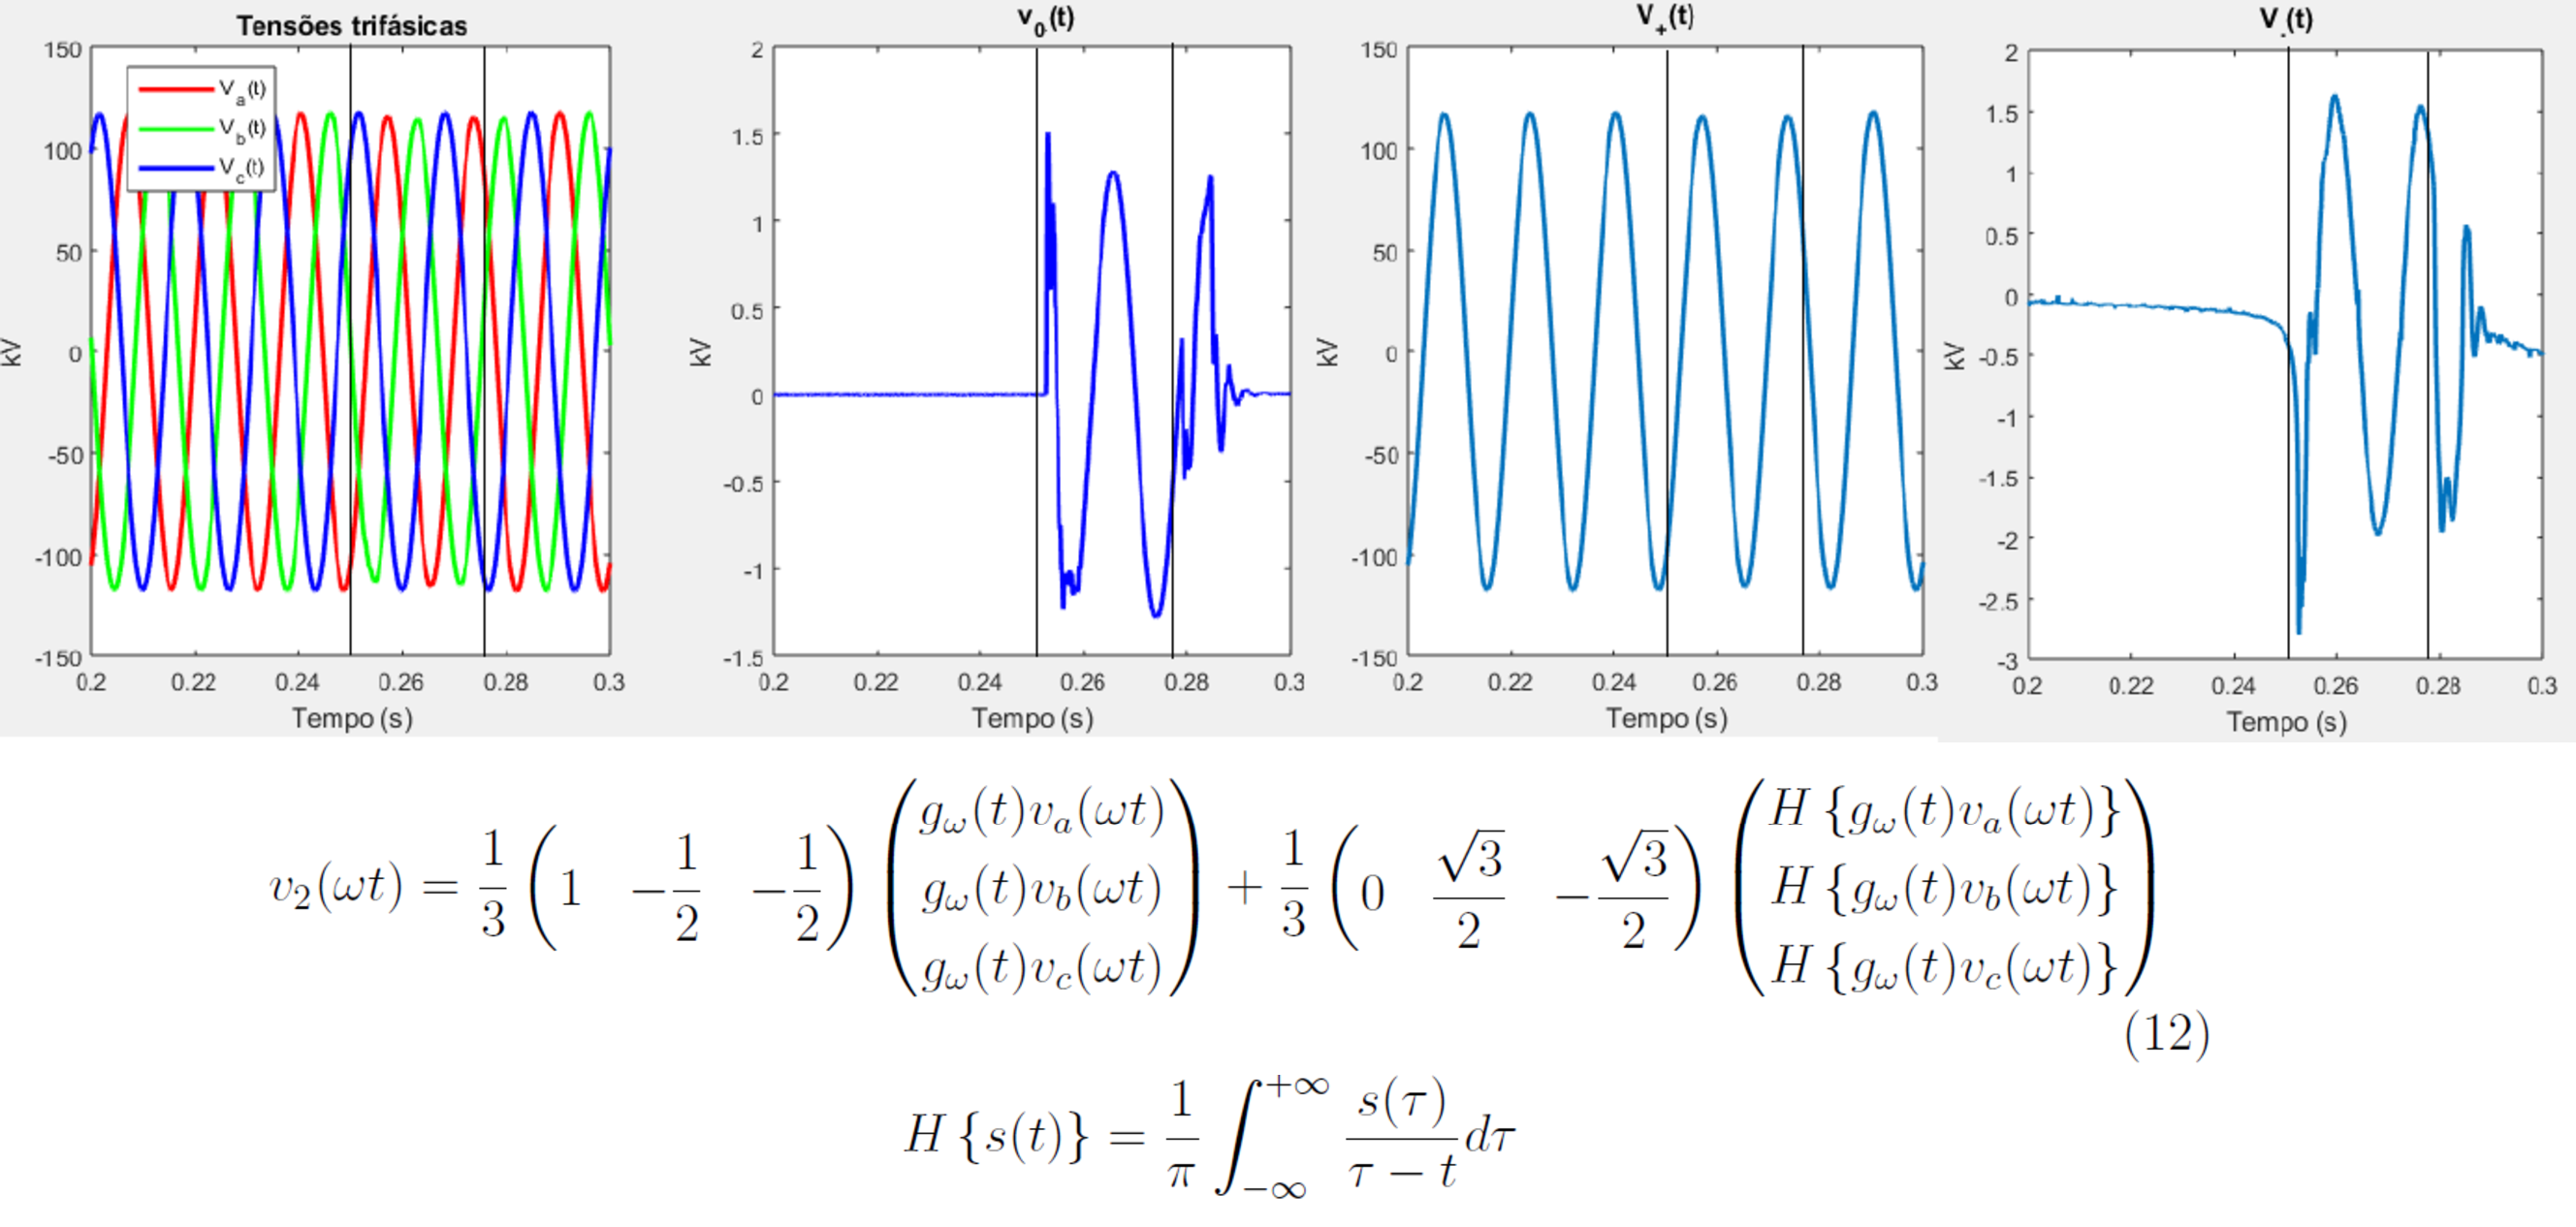
\includegraphics[width=0.65\linewidth]{./figuras/Exportacao/ex_processamento}


\end{frame}






%%%%%%%%%%%%%%%%%%%%%%%%%%%%%%%%%%%%%%%%%%%%%%%%
%%%%%%%%%%%%%%%%%%%%%%%%%%%%%%%%%%%%%%%%%%%%%%%%
%%%%%%%%%%%%%%%%%%%%%%%%%%%%%%%%%%%%%%%%%%%%%%%%
%%%%%%%%%%%%%%%%%%%%%%%%%%%%%%%%%%%%%%%%%%%%%%%%
\begin{frame}{Primeira Possibilidade: Serve para Pequenas Tarefas}
\centering

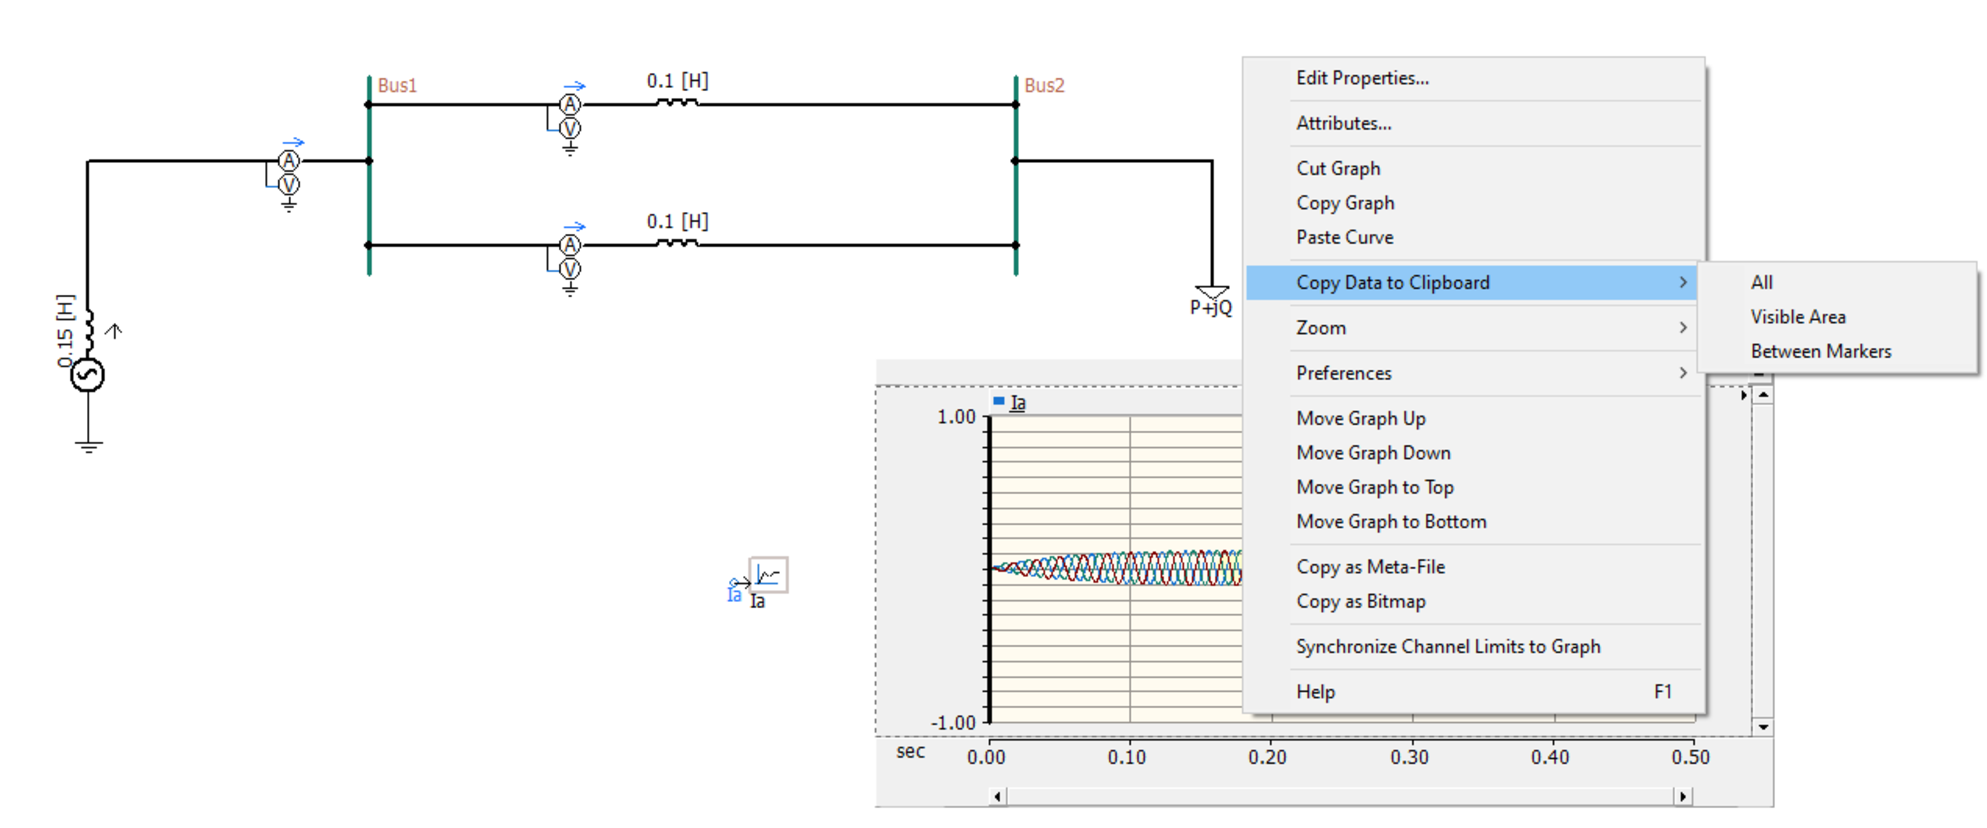
\includegraphics[width=0.95\linewidth]{./figuras/Exportacao/Export1}



\end{frame}




%%%%%%%%%%%%%%%%%%%%%%%%%%%%%%%%%%%%%%%%%%%%%%%%
%%%%%%%%%%%%%%%%%%%%%%%%%%%%%%%%%%%%%%%%%%%%%%%%
%%%%%%%%%%%%%%%%%%%%%%%%%%%%%%%%%%%%%%%%%%%%%%%%
%%%%%%%%%%%%%%%%%%%%%%%%%%%%%%%%%%%%%%%%%%%%%%%%
\begin{frame}{Primeira Possibilidade: Serve para Pequenas Tarefas}
\centering

É só colar em um arquivo de texto:

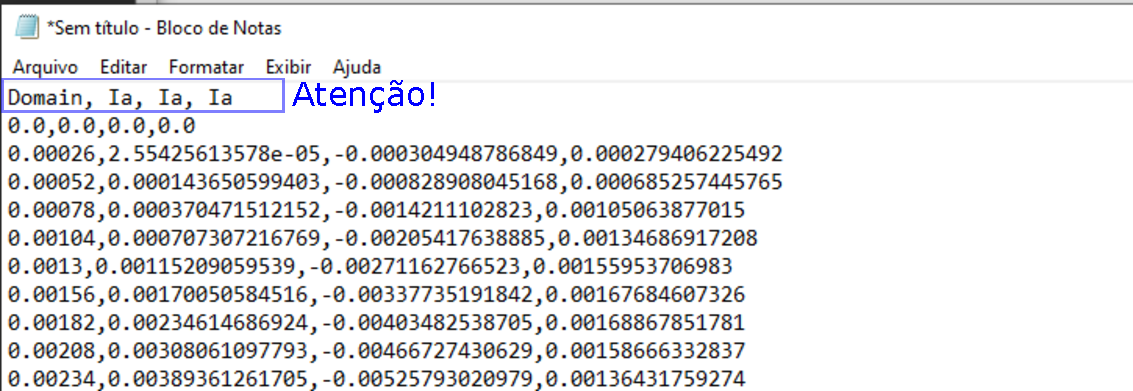
\includegraphics[width=0.95\linewidth]{./figuras/Exportacao/Export1-arquivo}



\end{frame}







%%%%%%%%%%%%%%%%%%%%%%%%%%%%%%%%%%%%%%%%%%%%%%%%
%%%%%%%%%%%%%%%%%%%%%%%%%%%%%%%%%%%%%%%%%%%%%%%%
%%%%%%%%%%%%%%%%%%%%%%%%%%%%%%%%%%%%%%%%%%%%%%%%
%%%%%%%%%%%%%%%%%%%%%%%%%%%%%%%%%%%%%%%%%%%%%%%%
\begin{frame}{Segunda Possibilidade: Útil para Grandes Tarefas}
\centering


\begin{columns}

\column{0.5\linewidth}
\begin{itemize}
\item Podemos configurar a simulação para salvar os dados dos {\i output chanels}
\vspace*{0.5cm}
\item Basta configurar a opção {\it save to disk}
\vspace*{0.5cm}
\item É gerado um arquivo com extensão {\color{blue}\it .map} contendo informações
\vspace*{0.5cm}
\item São gerados aquivos com extensão {\color{blue}\it .out} contendo os dados
\end{itemize}

\column{0.5\linewidth}
\centering
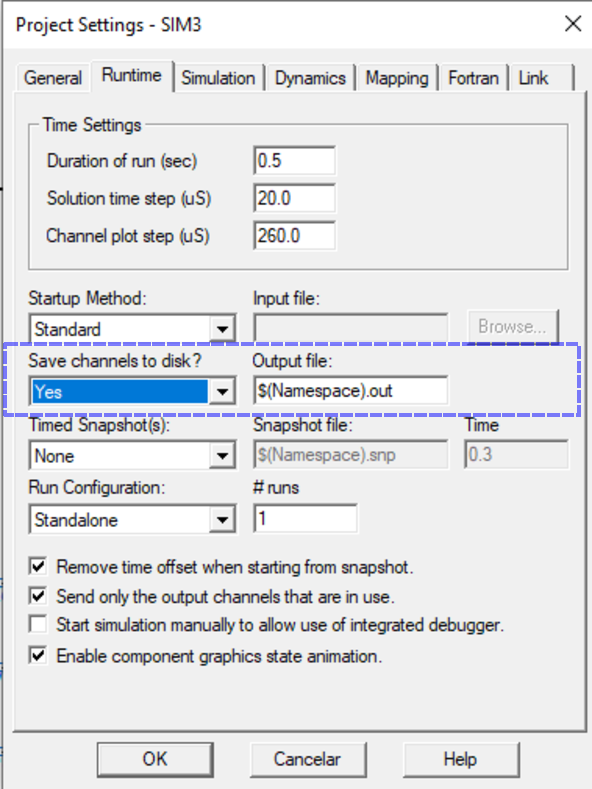
\includegraphics[width=0.70\linewidth]{./figuras/Exportacao/Export2}

\end{columns}


\end{frame}







%%%%%%%%%%%%%%%%%%%%%%%%%%%%%%%%%%%%%%%%%%%%%%%%
%%%%%%%%%%%%%%%%%%%%%%%%%%%%%%%%%%%%%%%%%%%%%%%%
%%%%%%%%%%%%%%%%%%%%%%%%%%%%%%%%%%%%%%%%%%%%%%%%
%%%%%%%%%%%%%%%%%%%%%%%%%%%%%%%%%%%%%%%%%%%%%%%%
\begin{frame}{Segunda Possibilidade: Útil para Grandes Tarefas}
\centering


\begin{columns}

\column{0.5\linewidth}
\begin{itemize}
\item Os arquivos {\color{blue}\it .out} e {\color{blue}\it .map} são dispostos na pasta de arquivos compilados da simulação
\vspace*{1cm}
\item Cada arquivo {\color{blue}\it .out} têm até 10 sinais, um por coluna
\vspace*{1cm}
\item A primeira coluna de todos os arquivos {\color{blue}\it .out} contém o vetor de domínio (Tempo ou Frequência)  
\end{itemize}

\column{0.5\linewidth}
\centering
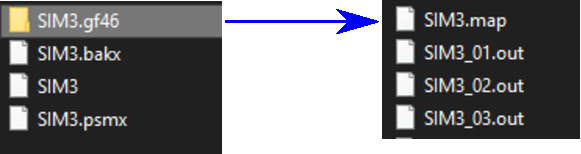
\includegraphics[width=0.70\linewidth]{./figuras/Exportacao/Export2-files}


\end{columns}


\end{frame}






%%%%%%%%%%%%%%%%%%%%%%%%%%%%%%%%%%%%%%%%%%%%%%%%
%%%%%%%%%%%%%%%%%%%%%%%%%%%%%%%%%%%%%%%%%%%%%%%%
%%%%%%%%%%%%%%%%%%%%%%%%%%%%%%%%%%%%%%%%%%%%%%%%
%%%%%%%%%%%%%%%%%%%%%%%%%%%%%%%%%%%%%%%%%%%%%%%%
\begin{frame}{Segunda Possibilidade: Útil para Grandes Tarefas}
\centering


\begin{columns}

\column{0.5\linewidth}
\centering
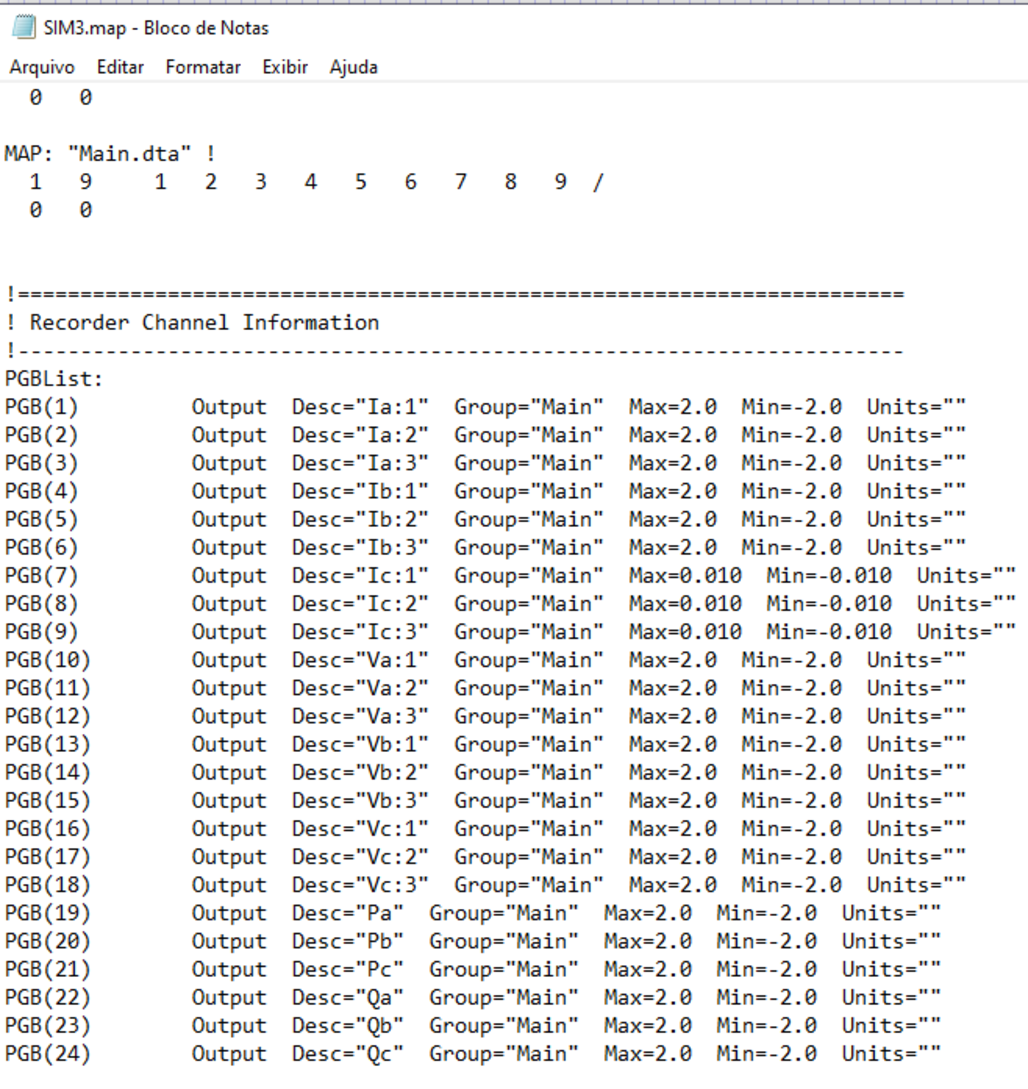
\includegraphics[width=0.80\linewidth]{./figuras/Exportacao/Export2-map}

\column{0.5\linewidth}
\centering
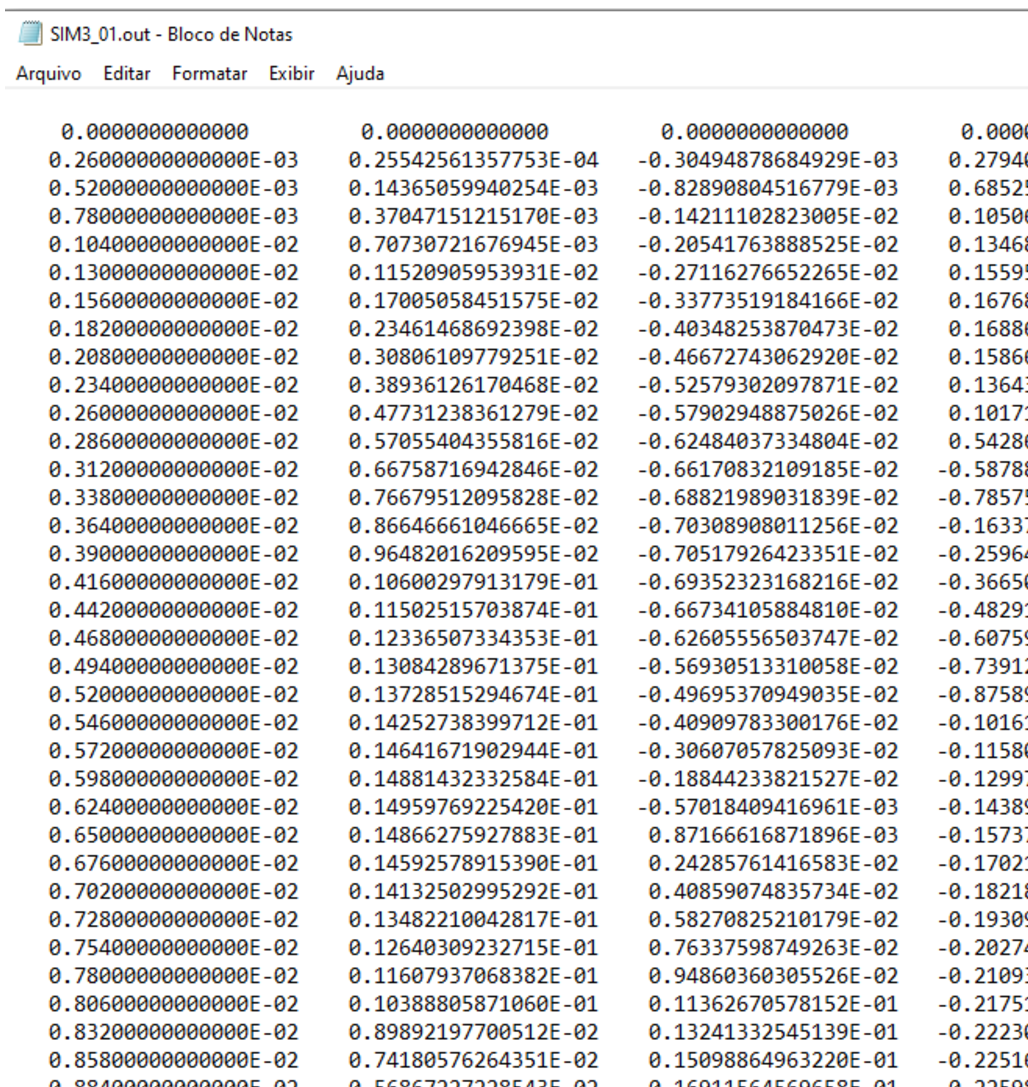
\includegraphics[width=0.80\linewidth]{./figuras/Exportacao/Export2-out}


\end{columns}


\end{frame}


